
%(BEGIN_QUESTION)
% Copyright 2013, Tony R. Kuphaldt, released under the Creative Commons Attribution License (v 1.0)
% This means you may do almost anything with this work of mine, so long as you give me proper credit

This pictorial diagram shows the wiring connections for a simple pressure control loop, where a loop-powered 4-20 mA pressure transmitter sends a signal to a Honeywell controller, which in turn sends another 4-20 mA signal to a control valve:

$$\includegraphics[width=15.5cm]{i02696x01.eps}$$

If an operator informs you that the pressure indicated by the Honeywell controller is below range (``pegged'' full downscale, reading -10\%), what types and locations of electrical faults might you suspect?  Are there any non-electrical faults which might also cause this to happen?


\underbar{file i02696}
%(END_QUESTION)





%(BEGIN_ANSWER)

If the Honeywell controller is pegged downscale, it means the analog input is receiving too little voltage.  A failed-open cable anywhere from the controller to the transmitter would do this, as would a dead DC power supply.
 
\vskip 10pt

No fault in the valve (output) circuit would have any effect on the controller's indication of pressure, since the valve control circuit is independent of the transmitter circuit.

%(END_ANSWER)





%(BEGIN_NOTES)


%INDEX% Pictorial circuit review (4-20 mA loop)
%INDEX% Troubleshooting review: electric circuits

%(END_NOTES)


